\documentclass[conference]{IEEEtran}
\usepackage{array,tabularx}
\usepackage{graphicx,xcolor,float}
\graphicspath{{./}{Lab4/}}
\usepackage[caption=false,font=footnotesize]{subfig}
\usepackage[hidelinks]{hyperref}
\newcommand{\designfolder}{\url{https://drive.google.com/drive/folders/1t8vxX2LX5kcBLTqoLPOU7HXXxWSGfxTj}}

% Fill in the placeholders. Add table rows as needed.
\renewcommand{\thesection}{\arabic{section}}
\newcolumntype{Y}{>{\raggedright\arraybackslash}X}
\renewcommand{\arraystretch}{1.25}
\newcommand{\fillin}[1]{\textcolor{gray}{\textit{[#1]}}}
\newcommand{\entry}[2]{\par\medskip\noindent\textbf{#1}\par\fillin{#2}\par}
\newcommand{\blank}{\fillin{---}}
\newcommand{\figureplaceholder}[1]{\fbox{\parbox[c][1in][c]{0.92\linewidth}{\centering\fillin{#1}}}}


% Photos may be compiled from the Lab4 folder or repository root.
\newcommand{\reportphoto}[2][\linewidth]{%
    \IfFileExists{images/#2}{%
        \includegraphics[width=#1]{images/#2}%
    }{%
        \IfFileExists{Lab4/images/#2}{%
            \includegraphics[width=#1]{Lab4/images/#2}%
        }{%
            \figureplaceholder{Add photo: \detokenize{#2}}%
        }%
    }%
}

\title{Lab 4: Design, Prototyping, and Anthropomorphization\\
\large INFO 5356: Introduction to Human-Robot Interaction}
\author{
\IEEEauthorblockN{Elliot Zhang, Yifan (Fanning) Luo, Jaclyn Pham, Jiaxin (Aurora) Shen}
\IEEEauthorblockA{Cornell Tech\\
\{qz432, yl4389, cqp4, js3996\}@cornell.edu}
}

\begin{document}
\maketitle


\section{Introduction}

Disco Moo is an educational human-robot interaction game designed to introduce K--12 students, particularly middle school learners, to foundational programming concepts through tangible, block-based coding. Inspired by Scratch, the game transforms conventional screen-based programming into a physical activity in which students assemble 3D-printed coding blocks to control a cow-themed Reachy Mini robot.

Each block represents a programming instruction, such as turning the robot's head, performing a movement, or repeating an action. The system uses ArUco markers to visually recognize and interpret commands; the physical blocks are designed to carry these markers. During gameplay, Reachy presents a dance challenge, and students construct a sequence of blocks to produce the requested movements. Through a camera-based interface, the program can be scanned and executed by Reachy, providing a physical demonstration of the relationship between code and robotic behavior.

The game primarily focuses on three computational thinking concepts: sequencing, repetition, and debugging. By arranging, testing, and revising physical instructions, students can explore how programming logic translates into observable actions without needing prior experience writing Python code. The design also creates opportunities for collaborative problem-solving and progressive learning, informed by feedback from a K--12 teacher panel.

For Lab 4, our team developed a preliminary functional prototype, including 3D-printed interlocking coding blocks, paper-based ArUco marker recognition, a camera-based execution interface, and a customized cow-inspired robot embodiment. These components establish the foundation for further integration and evaluation in the final project.



\section{Teacher Interviews}

\subsection{Interview Questions and Responses}

Our team participated in the K--12 Teacher Panel on October 28, 2026, to gather educators' perspectives on designing an interactive robotic game for middle school students. We collected notes from five teachers.

\textbf{Data collected.} In total, five teachers took part. We recorded written notes during the session and conducted our thematic analysis on the panel transcript (Section~\ref{sec:thematic}). We presented Disco Moo as our proposed game. In it, students use physical coding blocks to program a cow-themed Reachy Mini to perform dance sequences, with the goal of introducing foundational programming concepts through tangible, embodied, and collaborative learning.

We prepared four questions to understand students' programming experiences, common learning challenges, and opportunities for integrating physical robotics into computer science education:

\begin{enumerate}
    \item What CS courses or topics do you teach to middle school students, and at which grade levels?
    \item Which programming languages, platforms, or tools do your students use?
    \item Which programming concepts do you teach, and which do students find most challenging?
    \item How could physical coding blocks and a moving robot support the concepts you teach? Which concepts seem like the best fit, and why?
\end{enumerate}

The teachers discussed Scratch, block-based programming, and Python as common tools for introducing programming concepts. They emphasized that students should develop foundational computational thinking skills rather than rely solely on AI-assisted coding tools.

Teachers also highlighted the importance of breaking complex programming tasks into manageable steps. Visual and verbal instructions were recommended to support students with different learning needs, including English language learners and students with disabilities.

Regarding feedback, teachers recommended providing specific, encouraging hints instead of immediately revealing correct answers. They also emphasized collaborative activities and rotating student roles to ensure participation when classroom access to robots is limited.

Finally, teachers stressed that educational robotics activities should align with curriculum objectives and remain feasible within classroom time and resource constraints.

Table~\ref{tab:responses} summarizes the responses by question. The last three rows came up in the broader panel discussion, including other students' questions, rather than as direct answers to our four questions.

\begin{table}[t]
\centering
\caption{Summary of teacher panel responses}
\label{tab:responses}
\begin{tabularx}{\columnwidth}{>{\raggedright\arraybackslash}p{0.27\columnwidth} Y}
\hline
\textbf{Question / topic} & \textbf{Panel responses} \\
\hline
Q1--Q2: Courses and tools & Block-based programming, Scratch, and Python in middle- and high-school classes; some environments let students move between blocks and Python. Students should understand code ``under the hood,'' not only AI-generated code. \\
Q3: Concepts and challenges & Introductory games can teach the structure of instructions, including loops and conditionals. Large, open-ended tasks are hard; break work into ``very distinct chunks.'' \\
Q4: Fit of blocks and robot & Tangible blocks make instruction structure accessible. The robot should make a program's result visible and tie it to an identifiable skill, not serve only as a demo. \\
Feedback on mistakes & Specific, encouraging hints instead of ``that's wrong, the answer is X''; point to one area to improve. \\
Collaboration & One robot means waiting and possible domination by confident students; rotate roles and build turn-taking ``into the rules.'' \\
Curriculum and logistics & The game should add ``an extra bump'' to the curriculum, not ``pretty parts and pieces''; consider class time, preparation, group size, and reusable materials. \\
\hline
\end{tabularx}
\end{table}

\subsection{Thematic Analysis}
\label{sec:thematic}

Two team members, Jiaxin Shen and Yifan Luo, served as independent coders. We conducted an inductive thematic analysis of the October 28 teacher panel transcript. Each coder identified excerpts that bore on the design of Disco Moo and assigned a short descriptive code to each one. The codes concerned learning objectives, accessibility, feedback, engagement, and classroom participation. We then compared codes, discussed differences in interpretation, and grouped related codes into themes. We did not limit coding to our four interview questions. Five themes were especially relevant to the design.

\begin{enumerate}
    \item \textbf{Make computational thinking visible.} Panelists described block coding and Python as common approaches in middle- and high-school classrooms. One teacher emphasized helping students understand what happens ``under the hood'' rather than relying entirely on AI-generated code. Another noted that introductory games can teach the structure of instructions, including loops and conditionals. These comments shaped how we use tangible coding blocks. Reachy's movements are meant to make the consequences of a sequence observable, so the program is not left hidden inside generated code.

    \item \textbf{Scaffold the activity, not just the code.} Teachers cautioned against presenting middle-school students with a large, open-ended project all at once. One recommended breaking work into ``very distinct chunks''; another stressed clear verbal and visual prompts. We therefore organized the dance missions so that each one introduces a single challenge, with instructions available in more than one form.

    \item \textbf{Treat errors as opportunities to revise.} Panelists favored robot feedback that offers clues rather than the answer. As one put it, the robot should not respond with ``that's wrong, the answer is X.'' They also recommended keeping feedback specific and encouraging. We therefore moved away from ending a student's turn after an incorrect sequence. The proposed interaction uses robot prompts and interface cues that help students inspect, test, and revise their program.

    \item \textbf{Design participation into the rules.} Teachers warned that one student may dominate a shared game, particularly when they grasp the task more quickly than a partner. They suggested rotating roles and building turn-taking ``into the rules of your activity.'' We accordingly shifted from isolated individual turns toward collaborative planning, block assembly, testing, and debugging, with roles that can rotate across a mission.

    \item \textbf{Make classroom value and logistics explicit.} Panelists repeatedly asked whether a robotic game would strengthen the curriculum rather than merely attract attention. One teacher asked whether it would give the curriculum ``an extra bump'' or amount to ``pretty parts and pieces.'' They also raised preparation time, how many students would share a robot, and the need for ready-to-use materials. Disco Moo therefore has to make its programming objectives legible to teachers and include a practical plan for group rotation and for work away from the robot.
\end{enumerate}

Together, these themes suggest that an engaging robot is not, by itself, an educational activity. For Disco Moo, the design problem is to connect the appeal of robot movement to a visible programming sequence, a manageable progression of tasks, useful chances to revise, and a participation structure that works in a classroom. Our proposed interface will display the interpreted program and offer debugging cues, and Reachy Mini will give encouraging, hint-based responses. These are design intentions informed by the panel, not outcomes the panel established. Whether they improve learning or participation remains to be evaluated.

Table~\ref{tab:themes} condenses each theme into its design implication.

\begin{table}[t]
\centering
\caption{Themes and design implications for Disco Moo}
\label{tab:themes}
\begin{tabularx}{\columnwidth}{>{\raggedright\arraybackslash}p{0.33\columnwidth} Y}
\hline
\textbf{Theme} & \textbf{Design implication} \\
\hline
1. Make computational thinking visible & Prioritize sequencing, loops, and debugging; each block maps to a movement students can observe. \\
2. Scaffold the activity, not just the code & Progressive dance missions, each introducing one new concept, with instructions on screen and from Reachy. \\
3. Treat errors as opportunities to revise & Encouraging robot reactions and screen cues that point to the relevant step, instead of ending the turn. \\
4. Design participation into the rules & Small groups with rotating Planner, Builder, and Debugger roles. \\
5. Make classroom value and logistics explicit & An explicit programming objective per mission, short missions, and reusable blocks. \\
\hline
\end{tabularx}
\end{table}

\subsection{Influence on Robot and Game Design}
\label{sec:influence}

The panel moved our concept from a simple robot-command game toward a structured educational experience. In our original concept, students took turns arranging coding blocks to complete movement challenges. Correct programs triggered celebratory robot behaviors. Incorrect programs produced disappointed reactions and ended the student's turn. Table~\ref{tab:influence} summarizes how the panel changed this design.

\begin{table}[t]
\centering
\caption{Design changes motivated by the teacher panel}
\label{tab:influence}
\begin{tabularx}{\columnwidth}{>{\raggedright\arraybackslash}p{0.19\columnwidth} Y Y}
\hline
\textbf{Aspect} & \textbf{Initial concept} & \textbf{Revised design (theme)} \\
\hline
Game format & Individual turns; a mistake sends the student to the back of the line & Small groups with rotating roles (4) \\
Mistakes & Disappointed reaction; turn ends & Encouraging reaction, hint, retry (3) \\
Progression & Single-level movement challenges & Missions from sequences to loops to free choreography (2) \\
Instructions & Spoken challenge from Reachy & Screen shows the mission and interpreted program; Reachy acts it out (1, 2) \\
Learning goal & Implicit in the challenge & Explicit objective per mission (5) \\
\hline
\end{tabularx}
\end{table}

\textbf{Game behavior.} Three changes matter most. First, we shifted from elimination-based to collaborative gameplay. Students work in small groups, rotate roles, and debug together instead of losing their turn after a mistake. Second, we introduced progressive learning objectives and constructive feedback. Each mission targets a specific programming concept, and errors become opportunities for reflection and revision. Third, we incorporated multimodal feedback. The screen displays the target choreography, the interpreted program, and debugging hints, while Reachy physically demonstrates the movements.

\textbf{Robot behavior and embodiment.} The panel's emphasis on encouraging feedback also shaped Reachy's persona. A friendly, slightly clumsy cow makes an incorrect program feel like a dance step to fix together rather than a wrong answer (Section~\ref{sec:role}). These changes strengthen the game's educational purpose while keeping its playful character.

\subsection{Reflection}

The teacher panel helped us recognize that designing an educational robotic game involves more than selecting programming concepts. Although our original questions were useful for understanding classroom programming tools and learning difficulties, the discussions revealed additional considerations related to accessibility, student participation, and constructive feedback.

One important lesson was the distinction between making a robot entertaining and making it educational. While Disco Moo's cow-themed appearance and expressive dance movements may increase engagement, the gameplay must also provide opportunities to practice identifiable programming skills.

The panel also challenged our initial assumption that individual turn-taking would be an effective classroom format. Teachers highlighted the importance of keeping students engaged even when they are not directly controlling the robot, encouraging us to explore rotating roles and collaborative debugging.

In future interviews, we would ask more specific follow-up questions about appropriate challenge duration, group size, and methods for evaluating students' understanding of sequencing and loops. Presenting a storyboard or functional prototype could also help teachers provide more concrete feedback on the interaction design.

\textbf{Question suitability.} Our four questions worked well for learning which tools and concepts teachers already use. They did not ask about feedback, participation, or classroom logistics. Those topics came up only through follow-up discussion and other students' questions, yet they produced most of our design changes. Probing questions we would add include:
\begin{itemize}
    \item How long should one mission last to fit a class period?
    \item How many students should share one robot and one set of blocks?
    \item How do you check whether students understand loops and sequencing?
    \item What should students who are waiting for the robot do in the meantime?
\end{itemize}
We have since drawn the storyboard in Fig.~\ref{fig:storyboard}, which we plan to bring to future teacher conversations.



\section{Robot Concept and Design Process}
\label{sec:designprocess}

\subsection{Robot Role and Embodiment}
\label{sec:role}

Disco Moo is a tangible programming game in which Reachy Mini acts as both a playful dance partner and an interactive coding companion. Inspired by Scratch, the game allows students to construct programs by physically assembling modular coding blocks instead of typing commands on a computer. Each block represents an instruction, such as turning the robot's head, nodding, or repeating a movement.

During gameplay, Reachy presents a dance challenge that students must solve by arranging the appropriate blocks in sequence. For example, Reachy might ask students to make it turn left, nod twice, and turn right. Students select and connect the corresponding blocks, present their program to the camera, and press Scan to start recognition and execution. Reachy's physical movements provide an observable representation of the programmed instructions, helping students understand sequencing and repetition.

Reachy is designed with a friendly, cow-inspired persona to make the interaction more playful and approachable for younger learners. We created a felt-backed coat with white yarn and black patches to establish a cow-like appearance while keeping Reachy's head visible. The robot's character is reflected in its dance-oriented challenges and planned encouraging feedback. Rather than functioning solely as a device that executes commands, Disco Moo is intended to act as a learning companion that encourages experimentation and collaborative problem-solving.

Based on the teacher panel feedback, we revised our initial individual turn-taking concept toward collaborative gameplay. Students can work together to plan sequences, assemble blocks, test their programs, and identify errors. The proposed interaction also includes progressively challenging missions and supportive feedback, allowing students to practice fundamental programming concepts without requiring prior Python experience.

\textbf{Interaction role.} Reachy Mini serves as an embodied learning companion and performer, not a strict instructor or evaluator. Its job is to make abstract programming concepts observable through movement, while encouraging students to experiment, collaborate, and learn from mistakes. Students help choreograph Disco Moo, an enthusiastic dancing cow, so the activity has a concrete purpose: they are not simply executing commands but helping a character complete dance missions.

\textbf{Persona.} We designed Disco Moo as a friendly, curious, and slightly clumsy cow. This personality supports an approachable environment in which students feel comfortable experimenting and making mistakes. Because Reachy depends on the students' instructions to dance, the game gives students agency over the robot, and debugging feels like helping a character rather than correcting a failure.

\textbf{How the embodiment supports the role.} The soft white yarn, irregular black spots, and rounded silhouette communicate warmth and friendliness, and the recognizable dairy-cow pattern gives the character a memorable identity. Rather than replacing Reachy Mini's form, the coat builds on it. The wide head, circular eyes, and flexible antennas stay visible, so Reachy can still communicate through gaze, head tilts, nodding, and antenna movement. The persona shapes these expressive behaviors. Reachy wiggles its antennas and dances after a successful program, and tilts its head curiously when students need to debug. Playful sound effects reinforce the character. The coding blocks repeat Reachy's glasses motif, so the objects students hold visibly belong to the same character.

\subsection{Storyboard and Interaction Flow}
\label{sec:storyboard}

We used storyboarding as our first design method to plan how a group of students would play one mission. Fig.~\ref{fig:storyboard} shows the six panels, which we drew after the teacher panel so that they reflect the revised, collaborative game.

\begin{figure*}[t]
    \centering
    \reportphoto[0.82\textwidth]{storyboard.jpg}
    \caption{Storyboard of one Disco Moo mission. Left column, top to bottom: Disco Moo introduces a dance challenge while the screen shows the target sequence; students arrange the physical coding blocks together; Reachy performs the programmed dance with sounds and expressive movements. Right column: students take the Planner, Builder, and Debugger roles; Reachy scans the blocks and the computer shows the interpreted program; if the sequence is incorrect, Reachy gives a hint, the screen marks the step to revise, and students try again.}
    \label{fig:storyboard}
\end{figure*}

The storyboard defines five interaction stages:
\begin{enumerate}
    \item \textbf{Challenge presentation.} Disco Moo introduces a dance mission, and the screen displays the target movement sequence.
    \item \textbf{Role assignment and collaborative programming.} Students take the Planner, Builder, and Debugger roles and arrange the physical command blocks together.
    \item \textbf{Program recognition.} Reachy's camera captures the block arrangement, and the computer displays the interpreted program.
    \item \textbf{Execution and feedback.} Reachy performs the programmed movements with sounds, while the screen highlights the step in progress.
    \item \textbf{Debugging and progression.} If the sequence does not match, Reachy gives a hint and the screen marks the step to check, without revealing the answer. Students revise the blocks and retry, or advance to a harder mission.
\end{enumerate}

The planned difficulty progression begins with short movement sequences, introduces repeated actions through loops, and ends with students creating their own choreography. Roles rotate between missions so that every student plans, builds, and debugs.

\subsection{Expected Behaviors and Student Needs}
\label{sec:behaviors}

Reachy's primary movements are head turning, nodding, head shaking, antenna gestures, and body rotation. Each corresponds directly to a coding block, so students can compare their instructions with the robot's behavior. Table~\ref{tab:behaviors} maps each expected behavior to the student need it addresses. Stages 3 and 4 have been demonstrated with paper markers (Section~\ref{sec:addoutput}). The mission display, hints, and encouraging error reactions are planned for the final project.

\begin{table}[t]
\centering
\caption{Expected robot behaviors and the student needs they address}
\label{tab:behaviors}
\begin{tabularx}{\columnwidth}{>{\raggedright\arraybackslash}p{0.38\columnwidth} Y}
\hline
\textbf{Behavior} & \textbf{Student need (theme)} \\
\hline
Perform each block as a movement, one step at a time & See how program order produces behavior (1) \\
Highlight the active step on screen beside the robot & Link instructions to actions; visual support for diverse learners (1, 2) \\
Introduce missions verbally and on screen & Clear, multimodal instructions; one new concept at a time (2) \\
Head tilt, encouraging sound, and a hint on a mismatch & Clues instead of answers; safe to make mistakes (3) \\
Antenna wiggle and celebratory dance on success & Motivation and persistence \\
Prompt role rotation between missions & Equal participation with one robot (4) \\
\hline
\end{tabularx}
\end{table}

The screen complements Reachy's movements by displaying instructions, the program sequence, and debugging cues, which responds to the teachers' call for clear visual and verbal guidance. Rotating roles and a single shared block set address the teachers' concerns about limited robot access and one student dominating the activity.

\subsection{Iterative Design}

Our design process involved several stages of ideation, physical prototyping, and functional testing. We began with a Scratch-inspired game plan and with character studies for Reachy Mini. An early model dressed the robot as a jester, with a two-point hat, round glasses, and a small badge, as in Fig.~\ref{fig:jester-concept}. A follow-up sheet developed that model into front, side, back, three-quarter, top, and exploded views, and it still marked physical fit and range of motion as unchecked (Fig.~\ref{fig:jester-views}).

\begin{figure*}[t]
    \centering
    \subfloat[First character concept. Reachy wears a jester hat, round glasses, and a badge.]{%
        \includegraphics[width=0.40\textwidth]{"design process/Reachy logo first concept .png"}%
        \label{fig:jester-concept}}
    \hfil
    \subfloat[First character iteration. The same jester model is shown from the front, side, back, a three-quarter view, the top, and as an exploded set of parts.]{%
        \includegraphics[width=0.56\textwidth]{"design process/Reachy Logo first iteration.png"}%
        \label{fig:jester-views}}
    \caption{Early jester character studies for Reachy Mini, before the embodiment shifted toward a cow.}
    \label{fig:jester}
\end{figure*}

We then turned the embodiment toward a cow. The concept board in Fig.~\ref{fig:moobot} calls the character MooBot, a cow-themed Reachy Mini. It specifies a removable costume: 3D-printed horns, felt ears, a fabric collar with a bell, a spotted fleece cover, and a pom-pom tail. The board also records the constraints on any skin added to Reachy. Head tilt and rotation stay visible, the cover stays lightweight and removable, and it does not block the cameras or the antennas.

\begin{figure*}[t]
    \centering
    \includegraphics[width=0.98\textwidth]{"design process/Disco Moo concept.png"}
    \caption{Cow-themed embodiment concept for Disco Moo. The board shows the costume from several sides and separates 3D-printed parts, laser-cut parts, and the soft cover.}
    \label{fig:moobot}
\end{figure*}

For Reachy Mini's exterior, we developed the cow concept into a handmade felt-backed yarn coat. We attached white yarn and black patches with hot glue, then refined the fit using rows of retaining loops and adjustable cords. This material construction and fastening system are described in Section~\ref{sec:finaldesign}. The process let us work directly with Reachy's rounded body while keeping its recognizable head visible.

The black cow spots took their own iteration (Fig.~\ref{fig:spots}). Our first attempt tied short lengths of black yarn into small tufts, which looked more like pom-poms than cow markings (Fig.~\ref{fig:spots-materials}). We then drew irregular spot outlines on paper templates and coiled black yarn inside each outline to make flat, solid patches (Fig.~\ref{fig:spots-templates}). We arranged the finished patches on the white yarn surface to check size and placement before hot-gluing them on (Fig.~\ref{fig:spots-assembly}). The templates let us try several shapes cheaply and keep the spots irregular, like a real dairy cow's.

\begin{figure*}[t]
    \centering
    \subfloat[Materials: white fluffy yarn, black yarn, and the first tufted spots on a paper template.]{%
        \reportphoto[0.27\textwidth]{cow_spots_materials.jpg}%
        \label{fig:spots-materials}}
    \hfil
    \subfloat[Spot outlines drawn on paper templates and filled with coiled black yarn, next to the black felt backing.]{%
        \reportphoto[0.43\textwidth]{cow_spots_templates.jpg}%
        \label{fig:spots-templates}}
    \hfil
    \subfloat[Placing the finished spots on the white yarn surface before hot-gluing them.]{%
        \reportphoto[0.27\textwidth]{cow_spots_assembly.jpg}%
        \label{fig:spots-assembly}}
    \caption{Iterating on the cow spots: from yarn tufts to template-shaped coiled patches attached to the coat.}
    \label{fig:spots}
\end{figure*}

The coding blocks went through a similar pass from sketch to rendered mockup. Our initial plan used color-coded blocks for head movements, antenna movements, body rotation, and repetition. Because only a few block colors were available, we planned for color to mark a command category while a printed label or symbol identifies the individual action. The sketches in Fig.~\ref{fig:block-sketch} divide each block into four faces: the command on the front, Reachy's eyes on the top, an ArUco marker on the back, and the connecting face on the bottom. The mockups in Fig.~\ref{fig:block-mockups} then compared two characters for that block. One wears a jester hood with bells. The other is a plain block with two black eyes and a central post for stacking. The blocks we printed, described in Section 4, kept the Reachy face and the vertical stack, and simplified the face into a glasses-like bridge with four studs.

\begin{figure*}[t]
    \centering
    \subfloat[Block sketches. Each drawing labels one face: front, top, back, or bottom.]{%
        \includegraphics[width=0.42\textwidth]{"design process/lego block sketch.png"}%
        \label{fig:block-sketch}}
    \hfil
    \subfloat[Rendered block mockups. A jester-hood version sits beside a plain block with Reachy's eyes and a stacking post.]{%
        \includegraphics[width=0.54\textwidth]{"design process/lego block mockups.png"}%
        \label{fig:block-mockups}}
    \caption{Development of the tangible coding block, from a four-face sketch to two character mockups.}
    \label{fig:blocks}
\end{figure*}

We used 3D modeling and physical prototyping to investigate the blocks' connection mechanism. In particular, we produced variations with socket dimensions of 14.00 mm, 14.01 mm, 14.02 mm, and 14.03 mm to evaluate how dimensional tolerances affect the fit between blocks. This process allowed us to consider both connection stability and ease of assembly.

In parallel, we explored ArUco markers as a method for translating physical block arrangements into executable robot instructions. We printed the markers on paper and successfully tested their recognition and corresponding Reachy Mini movements through a camera-based interface. Each card pairs the marker with a move name and the command Reachy will run. Fig.~\ref{fig:sample-marker} shows the card for look right. The interface includes a camera view and a Scan control for initiating execution. Although this established the feasibility of the recognition system, integrating the markers directly onto the 3D-printed blocks remains a future step.

The teacher panel also informed an important iteration in our interaction design. Our original game plan involved students completing challenges individually, with incorrect answers ending their turns. Following the teachers' recommendations, we shifted toward collaborative problem-solving, progressive challenges, and constructive feedback.

Throughout the process, we considered fabrication time, available materials, and technical feasibility. 3D printing allowed us to produce reusable, interlocking blocks with consistent geometry, while paper-based marker testing enabled us to evaluate the software before completing the physical integration. These decisions helped us develop a preliminary functional prototype within the lab timeframe while identifying areas for further refinement.

\subsection{Resource, Time, and Cost Constraints}
\label{sec:constraints}

\textbf{Robot capabilities.} As a tabletop robot, Reachy Mini is better suited to expressive head, antenna, and body movements than to navigation. We therefore chose a dance game in which its existing movements are the core of the interaction, rather than adding new actuators.

\textbf{Embodiment constraints.} The coat has to stay lightweight and removable and must not restrict neck movement, cover the camera, or interfere with the antennas and ventilation. We therefore kept the head uncovered and limited the coat to the body.

\textbf{Cost.} Felt, yarn, paper templates, and hot glue are inexpensive and easy to rework. They let us change the character's appearance without modeling or printing a new robot shell. The limited range of block colors led to the category-color plus label scheme described above.

\textbf{Time.} Within the lab timeframe, we tested recognition and execution with paper markers before attaching them to the blocks, so the software-to-robot pipeline could be validated while block printing and tolerance testing went on in parallel.



\section{Fabrication}
\label{sec:fabrication}

\subsection{Laser-Cut Nametag}

During the early stages of our design process, we explored giving Reachy Mini a character inspired by Olaf from \textit{Frozen}. We combined Reachy's recognizable head and antennas with Olaf-inspired features, including buttons, a carrot nose, and twig-like arms. Through iterative testing of the design's proportions, we refined the relative sizes and placement of these elements to create a balanced composition that retained Reachy's identity while introducing a familiar, playful character.

We translated this concept into a laser-cut nametag featuring the character alongside the word REACHY. The nametag was fabricated from a 3\,mm board made by pressing leftover 3D-printing material into a flat sheet. Its mixture of colors created a distinctive marbled surface, making the reclaimed material an integral part of the visual design. The lettering and character details were formed through cutting, allowing the colorful material and open spaces to define the composition.

The main fabrication challenge was cutting through the reclaimed sheet. Three cutting passes were needed to fully separate the component, giving us practical experience adapting the fabrication process to the material. The completed piece demonstrates how fabrication leftovers can be transformed into a visually distinctive object.

As our project developed toward the cow-inspired Disco Moo concept, the nametag remained an artifact of our earlier character exploration. It documents our process of testing recognizable character features, refining proportions, and exploring how material choices contribute to a robot's visual identity.

\begin{figure}[t]
    \centering
    \IfFileExists{images/reachy_olaf_nametag.jpg}{%
        \includegraphics[width=\linewidth]{images/reachy_olaf_nametag.jpg}%
    }{%
        \IfFileExists{Lab4/images/reachy_olaf_nametag.jpg}{%
            \includegraphics[width=\linewidth]{Lab4/images/reachy_olaf_nametag.jpg}%
        }{%
            \figureplaceholder{Insert photograph: reachy\_olaf\_nametag.jpg.}%
        }%
    }
    \caption{Laser-cut REACHY nametag from a 3\,mm reclaimed 3D-printing material sheet. The Olaf-inspired character combines Reachy's head and antennas with a carrot nose, buttons, and twig-like arms. The material's multicolored surface provides the decorative finish.}
    \label{fig:lasercutnametag}
\end{figure}

The design file for the nametag, \texttt{Reachy Name Tag.ai}, is available in our shared design folder: \designfolder.

% Fabrication design file: designs/Reachy_Name_Tag.ai

\subsection{Custom Laser-Cut Part: CODE Farmland Sign}

Following the development of Disco Moo's cow-inspired identity, we designed a freestanding \textit{CODE Farmland} sign to extend the theme into the surrounding game environment. The farm concept connects the robot's character with the coding activity, giving the experience a playful and recognizable setting.

We selected a 5\,mm wooden board because its natural appearance complements the farm theme. The design combines large lettering with a Reachy Mini face motif, making the title visually prominent while maintaining a clear connection to the robot. A separate base with slots and corresponding tabs on the sign provides a simple structure for upright display.

The sign combines laser cutting and engraving. Cutting defines the outer profile, the outlined \textit{CODE} lettering, and the base and connection features. Engraving adds the Reachy Mini face and the word \textit{Farmland}. The contrast between the cut geometry and engraved surfaces gives the design a clear visual hierarchy while preserving the wood's natural appearance.

Laser cutting offered a straightforward fabrication method for this component. For the flat sign and base, cutting sheet material directly was more suitable than building the same profiles layer by layer with 3D printing. We chose wood for a rigid display structure and a farm-like appearance rather than using a paper or yarn construction. Both the sign and its base could be produced from flat sheet material, with structural outlines and decorative details incorporated into the same workflow. The resulting piece combines prominent typography, a recognizable robot motif, and a material that reinforces the farm setting, creating a cohesive visual companion to Disco Moo.

\begin{figure}[t]
    \centering
    \IfFileExists{images/code_farmland_fabrication.jpg}{%
        \includegraphics[width=\linewidth]{images/code_farmland_fabrication.jpg}%
    }{%
        \IfFileExists{Lab4/images/code_farmland_fabrication.jpg}{%
            \includegraphics[width=\linewidth]{Lab4/images/code_farmland_fabrication.jpg}%
        }{%
            \figureplaceholder{Insert photograph: code\_farmland\_fabrication.jpg.}%
        }%
    }
    \caption{Fabrication of the CODE Farmland sign and slotted base from 5\,mm wood. Engraving forms the Reachy Mini motif and Farmland text, while laser cutting defines the profiles, CODE lettering, and connection features.}
    \label{fig:farmlandfabrication}
\end{figure}

The design file for the sign and base, \texttt{CODE\_Farmland\_Reachy\_80mm.ai}, is available in our shared design folder: \designfolder.

% Fabrication design file: designs/CODE_Farmland.ai
% Supplied photographs should be placed in Lab4/images/:
% reachy_olaf_nametag.jpg -- completed colorful nametag photograph
% code_farmland_fabrication.jpg -- wood sign in the laser cutter

\subsection{3D-Printed Components}

We designed and fabricated modular coding blocks inspired by Reachy Mini's physical appearance. Each block features a rounded rectangular white body with two black circular elements connected by a narrow bridge, resembling Reachy's distinctive glasses. This visual design creates a consistent identity between the robot and the physical programming interface.

Each block incorporates four cylindrical studs on its upper surface, allowing multiple blocks to be stacked vertically. This interlocking mechanism enables students to physically construct a sequence of programming instructions, translating abstract coding structures into tangible arrangements.

During prototyping, we experimented with four socket dimensions: 14.00 mm, 14.01 mm, 14.02 mm, and 14.03 mm. These variations were designed to investigate how small dimensional differences influence the fit and stability of the connections. The tolerance testing formed an important part of our iterative fabrication process, as the blocks needed to remain connected while still being easy for students to assemble and separate.

We chose 3D printing because it allowed us to fabricate three-dimensional, reusable components with consistent shapes and integrated connection features. Unlike laser cutting or simple cardboard construction, 3D printing enabled the rounded geometry and cylindrical interlocking structures to be produced as part of the block design.

The physical blocks are intended to incorporate printed programming labels and ArUco markers. Each marker corresponds to a specific command that can be recognized through the camera-based interface and translated into a robot movement. We successfully tested marker recognition and robot execution using paper-printed ArUco markers. However, the markers have not yet been integrated and tested directly on the 3D-printed blocks.

The resulting prototypes demonstrate the physical feasibility of the modular coding system and provide a foundation for integrating tangible programming with Reachy Mini's movements.

% Assembled blocks are shown in Fig.~\ref{fig:finalrobot}.
The 3D modeling and printing files for the coding blocks are available in the same shared design folder: \designfolder.

% TODO: Specify the selected socket dimension and test outcome.




\section{Final Robot Design and Reflection}
\label{sec:finaldesign}

\subsection{Final Prototype}

Our final Lab 4 prototype, Disco Moo, combines a cow-themed Reachy Mini with tangible programming blocks and a CODE Farmland display sign (Fig.~\ref{fig:finalrobot}). A handmade white yarn coat with black patches establishes the cow identity while retaining Reachy's recognizable head and face. The programming blocks repeat the robot's facial motif, and the wooden sign extends the farm theme into the surrounding activity space. Together, these components give the coding game a consistent character and setting.

We constructed the coat on a felt backing. First, we wrapped the felt around Reachy's body to establish its approximate shape. We then used hot glue to attach white yarn to the backing, building a soft outer surface, and added smaller black patches to create the cow pattern. The felt provides the supporting shape, while the yarn and patches provide the texture and visual identity.

\begin{figure}[t]
    \centering
    \reportphoto{disco_moo_final.jpg}
    \caption{Final Disco Moo prototype with its white yarn coat and black cow patches, surrounded by 3D-printed coding blocks and the CODE Farmland sign. The early multicolored REACHY nametag is also displayed with the fabrication artifacts.}
    \label{fig:finalrobot}
\end{figure}

\subsection{Design Methods and Iterations}

Our process combined visual concept development, physical prototyping, and fitting the prototype on the robot. The sketches, concept boards, and digital models described in Section~\ref{sec:designprocess} helped us explore character identities and coordinate the appearance of the robot and blocks. Early explorations included the Olaf-inspired nametag and the jester studies. The later cow concept developed into a soft costume and a farm-themed activity setting. In parallel, the storyboard in Fig.~\ref{fig:storyboard} worked out the interaction itself: how a group receives a mission, divides roles, scans its blocks, and debugs after Reachy's hint.

Physical prototyping let us investigate how the materials would actually conform to Reachy. An initial felt wrap established the coat's size, and applying the yarn in stages let us develop its coverage and appearance. Fitting the coat on the robot revealed a problem that was difficult to resolve through a flat outline alone: the fabric did not naturally follow the rounded body.

We therefore introduced an adjustable fastening system inspired by several belt-like rows. We glued multiple small retaining loops to the inside of the coat and threaded long cords through them. Adjusting the cords at different heights changes the coat's circumference and helps it conform to the body. This iteration transformed a simple wrap into an adjustable garment that can be fitted and repositioned on Reachy (Fig.~\ref{fig:costumeprocess}).

\begin{figure*}[t]
    \centering
    \subfloat[Material assembly. White yarn is attached to the felt backing with hot glue to build the coat's outer surface.]{%
        \reportphoto[0.48\textwidth]{cow_costume_materials.jpg}%
        \label{fig:costumematerials}}
    \hfil
    \subfloat[Internal fastening structure. Rows of small retaining loops guide the long cords used to adjust the fit around Reachy's rounded body.]{%
        \reportphoto[0.48\textwidth]{cow_costume_lacing.jpg}%
        \label{fig:costumelacing}}
    \caption{Physical fabrication and fitting iterations for the cow costume. The layered material construction creates the character's surface, while the internal cord system adjusts its fit.}
    \label{fig:costumeprocess}
\end{figure*}

\subsection{Materials, Resources, and Feasibility}

We assigned materials and fabrication methods according to each component's role. Felt was suitable for cutting and establishing the coat's initial shape, yarn provided the soft surface, and hot glue supported incremental assembly. These common craft materials allowed local changes during fitting without requiring a new full-body model or another complete print. The approach balanced material use and machine time with hands-on assembly within the lab timeframe.

The costume focuses on the body below Reachy's head, keeping its recognizable face and antennas visible. Head movement is central to the dance interaction, so the relationship between the coat's upper edge and the moving head was an important placement consideration. The adjustable cords let us refine the garment's fit rather than relying on a fixed circumference.

For the other components, 3D printing supported the blocks' volumetric connection features, while laser cutting and engraving supported the wooden sign's profiles and graphics. The reclaimed sheet used for the early nametag also gave leftover fabrication material a new visual role. These choices combined fabrication tools with hand assembly instead of requiring one manufacturing method for every component.

\subsection{Affordances, Materiality, and Interaction Dimensions}

The blocks' studs and connecting surfaces suggest stacking and assembly. Their ordered arrangement gives students a physical way to represent program order. For the person fitting the costume, the retaining loops and cords provide a direct adjustment mechanism: tightening or loosening the cords changes how the garment fits the robot.

Materiality contributes to both identity and use. The white yarn and contrasting black patches establish the cow character through color and texture. The soft coat, rigid printed blocks, and wooden sign create distinct tactile and visual qualities, corresponding to character appearance, program construction, and scene identification. The approachable character is a design intention that supports the playful learning setting.

The interaction spans physical manipulation, screen-based interpretation, and robot movement. Students arrange blocks to construct a program; the camera-based interface displays the recognized sequence; and Reachy's movements make the commands observable. Our paper-marker trials demonstrated the recognition-to-movement connection. The costume and sign provide a shared narrative setting for this interaction, while the blocks provide its tangible programming form.

\subsection{Selected Fabricated Component}

We select the 3D-printed modular coding block as the fabricated component supporting the overall embodiment and interaction concept. Figure~\ref{fig:finalrobot} shows the blocks alongside Reachy. Their repeated facial motif connects them visually to the robot, while their interlocking geometry supports physical program construction. As external interaction objects, they extend the robot's identity into the objects students manipulate during the game.

\subsection{Reflection on the Embodiment Process}

Making the coat showed us that designing a robot's appearance also involves designing how materials fit and fasten to its body. The felt wrap revealed a mismatch between a flat pattern and a rounded surface. Adding the rows of loops and adjustable cords turned that fitting problem into a structural design opportunity.

This experience demonstrated the value of physical prototyping alongside visual concept development. Making and fitting the garment exposed issues that a concept image alone could not resolve, and those observations directly informed the next iteration. The final cow coat therefore represents both a character design and a practical response to the robot's physical form.


\section{Discussion and Future Work}

\subsection{Additional Research Output}
\label{sec:addoutput}

In addition to the physical coding blocks and the robot embodiment, we developed a camera-based interface that reads an ordered stack of ArUco markers and sends the corresponding commands to Reachy Mini. This is the screen a student would use to check which program the camera recognized and which step Reachy is carrying out. The prototype is titled Reachy LEGO. Figures~\ref{fig:ui-states} and~\ref{fig:ui-execution} show it during a feasibility test with paper markers. Fig.~\ref{fig:sample-marker} shows one of those cards. The pattern is an ArUco marker from the \texttt{DICT\_6X6\_250} dictionary. Under it, the card prints the move name, the command \texttt{head.turn\_right()}, and the instruction to attach the card flat and facing the camera so that every marker in the stack remains visible.

\begin{figure}[t]
    \centering
    \includegraphics[width=0.78\linewidth]{"additional research output/sample ArUco marker.png"}
    \caption{Sample paper marker for look right. The card combines the ArUco pattern, the move name, the command sent to Reachy, and the placement instruction for the camera.}
    \label{fig:sample-marker}
\end{figure}

The screen has four parts: a status bar, a short instruction, a live camera view, and a Sequence panel. In the ready state, the status bar reads READY and reports that the interface is connected to Reachy. The instruction asks the student to hold the stack in front of Reachy and press Scan. Until that scan succeeds, the Sequence panel states that the scanned sequence will appear there, as in Fig.~\ref{fig:ui-ready}.

Pressing Scan moves the interface to RUNNING. Each detected marker is outlined and labeled in the camera view. The Sequence panel then lists the moves in order, placing a plain-language name beside the command sent to the robot, and highlights the step currently underway. In Fig.~\ref{fig:ui-running}, the recognized program is twist body right, look right, and shake head. The status line names the first of those moves while Reachy performs it, and the Scan control changes to Please wait so the stack is not read again mid-dance.

\begin{figure*}[t]
    \centering
    \subfloat[Ready state. The student holds a vertical stack of ArUco markers in view of the camera. The interface asks them to press Scan, and the sequence list is still empty.]{%
        \includegraphics[width=0.48\textwidth]{"additional research output/custom UI - hold up markers.jpg"}%
        \label{fig:ui-ready}}
    \hfil
    \subfloat[Running state. Detected markers are labeled on the camera view, and the sequence panel highlights twist body right as the move Reachy is performing.]{%
        \includegraphics[width=0.48\textwidth]{"additional research output/custom UI - scanning in process.jpg"}%
        \label{fig:ui-running}}
    \caption{Custom interface a student would see while presenting a paper marker stack to Reachy Mini.}
    \label{fig:ui-states}
\end{figure*}

The same display stays beside the robot while the sequence runs, so the highlighted line and the physical movement can be checked against each other. Fig.~\ref{fig:reachy-exec} shows Reachy Mini during that test. The interface is RUNNING a six-step sequence and highlights twist body right as the active step. The camera view shows the marker sheet used for that longer program, with each detected marker labeled.

When the last move finishes, the status changes to CELEBRATING and the interface reports that the dance is complete. The full program remains on screen, including the action keys for the recognized markers, as in Fig.~\ref{fig:ui-complete}.

\begin{figure*}[t]
    \centering
    \subfloat[Reachy Mini executing the highlighted step. The interface lists a six-step sequence and marks twist body right as the move in progress.]{%
        \includegraphics[width=0.48\textwidth]{"additional research output/Reachy execute order and indicate which steps .jpg"}%
        \label{fig:reachy-exec}}
    \hfil
    \subfloat[Complete state. The status bar reads CELEBRATING, the interface reports that the dance is complete, and the full three-step sequence remains visible.]{%
        \includegraphics[width=0.48\textwidth]{"additional research output/complete state.jpg"}%
        \label{fig:ui-complete}}
    \caption{Reachy Mini carrying out a scanned sequence while the interface indicates the active step, and the screen after the dance finishes.}
    \label{fig:ui-execution}
\end{figure*}

These trials show that the interface can read an ordered stack, display the interpreted program, and have Reachy execute the listed moves one step at a time. The markers in this test were printed on paper. Attaching them to the 3D-printed blocks, and keeping each marker visible to the camera once those blocks are stacked, remains future work. For the selected fabricated component, we retain the 3D-printed modular coding block discussed in Section~\ref{sec:finaldesign}. Its interlocking structure and recognizable visual design provide the physical foundation for the proposed programming interaction.



\subsection{Reflection}

Developing Disco Moo helped us understand how physical fabrication, interaction design, and educational objectives must work together in human-robot interaction. One of our main challenges was translating abstract programming concepts into physical objects that are both intuitive to assemble and technically recognizable.

The laser-cut components also demonstrated how material choice shapes fabrication and visual identity. The reclaimed 3\,mm sheet gave the early Olaf-inspired nametag a distinctive multicolored appearance and required three cutting passes. For the CODE Farmland sign, 5\,mm wood reinforced the farm aesthetic, while combining cutting and engraving allowed structural and decorative features to be developed within one fabrication workflow. Together, the two pieces record how our character concepts and material choices evolved throughout the project.

The iterative fabrication process highlighted the importance of small dimensional adjustments in 3D printing. Testing different socket tolerances demonstrated how physical connection design can influence the usability of modular learning tools. Meanwhile, the paper-based ArUco tests allowed us to verify the basic software-to-robot interaction before completing the physical integration.

The teacher panel also significantly influenced our design approach. Initially, we focused on creating an entertaining individual coding challenge. However, the teachers' feedback encouraged us to consider scaffolding, accessibility, collaboration, and constructive feedback as essential components of an educational experience. This shifted our focus from simply making Reachy perform movements toward helping students understand the programming logic behind those movements.

Despite these developments, the current prototype has several limitations. Although ArUco recognition and robot execution were successfully tested using paper markers, the complete system has not yet been evaluated with markers attached to the 3D-printed blocks. Additionally, the proposed collaborative gameplay, progressive challenges, and debugging feedback require further implementation and testing.

For the final project, we plan to integrate ArUco markers and programming labels onto the physical blocks, refine the recognition of assembled command sequences, and further develop the interactive game interface. We also aim to evaluate whether students can understand sequencing, repetition, and debugging through the tangible coding experience. These next steps will help us move from a preliminary functional prototype toward a more complete educational robotic game.


\end{document}

